\documentclass[12pt,a4paper]{article}
\usepackage[utf8]{inputenc}
\usepackage{amsmath}
\usepackage{amsfonts}
\usepackage{amssymb}
\usepackage{lipsum}
\usepackage{textcomp}

\usepackage{makecell} % linebreak dans une cellule
\usepackage{multicol} % twocols localement
\usepackage{vwcol} % idem mais avec largeur variable
\usepackage{color, colortbl} % colorer les tableaux
\usepackage{enumitem} % utiliser des lettres pour énumérer
\usepackage{wrapfig} % insérer des images dans dutexte
\usepackage{dashundergaps} % transformer du texte en ________
\usepackage{MnSymbol,wasysym} % smileys
\usepackage{minibox} % multiline fbox - \minibox[frame]{}
\usepackage{ifthen}

% --- geometry ---
\usepackage{geometry}
\geometry{legalpaper, margin=1cm}
% ---

% --- xcolor ---
\usepackage{xcolor}
\definecolor{lightgray}{gray}{0.9}
% ---

% --- tcolorboxes ---
\usepackage[most]{tcolorbox}
\newtcolorbox{definition}[2][]{%
  attach boxed title to top left
               = {yshift=-8pt},
  colback      = white,
  colframe     = gray,
  fonttitle    = \bfseries,
  colbacktitle = gray,
  title        = #2,#1,
  enhanced,
}
% ---


\renewcommand{\baselinestretch}{1.15} % augmenter l'interligne

\dashundergapssetup{
	teacher-gap-format=underline,
	gap-widen
}



\author{Paul Clavier}
\title{Chapitre 1 - Tableaux et graphiques - Interrogation Écrite} 

\begin{document}

% --- Section & subsection renum ---
\renewcommand\thesection{\Roman{section}}
\renewcommand\thesubsection{\arabic{subsection}}
% ---

% --- Selection manuelle de la version ---
%\TeacherModeOn
% ---

% --- Selection automatique de la version ---
\ifdefined\isprof
	\TeacherModeOn
\fi

% ---

\begin{center}
	\minibox[frame,c]{Chapitre 1 - Tableaux et graphiques \\ Interrogation Écrite - 1}
\end{center}

\begin{center}
\begin{tabular}{|l|c|}
\hline \rowcolor{lightgray}
Organisation et gestion de données \hspace{8cm} & Maitrise \\ \hline
\thead[l]{1.1 : Prélever et organiser les informations nécessaires à la résolution de problèmes à partir de supports\\ variés : textes, tableaux, diagrammes, graphiques, dessins, schémas.} &
\\ \hline
\thead[l]{2.1 : Utiliser les mathématiques pour résoudre quelques problèmes issus de situations\\ de la vie quotidienne.} &
 \\ \hline
\end{tabular}
\end{center}

\textbf{Exercice 1}
En utilisant le tableau regroupant quelques villes, leur altitude, la quantité de pluie tombée en un an et le nombre de jours de pluie en un an ci dessous, répond aux questions.\\

\begin{minipage}{0.35\textwidth}
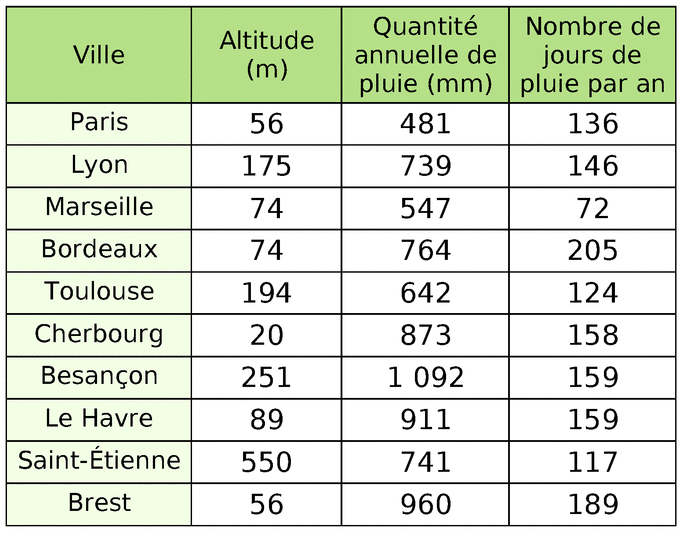
\includegraphics[scale=0.28]{img/IE-tableau.png} 
\end{minipage}
\begin{minipage}{0.5\textwidth}
\begin{enumerate}
\item Quelle est la ville la plus haute?\\ \gap*{Saint-Étienne\hspace{4.3cm}} 
\item Quelles sont les villes dont le nombre de jour de pluie est inférieur à 150?\\ \gap*{Paris, Lyon, Marseille, Toulouse, Saint-Étienne\hspace{4.5cm}}
\item Quelle ville à connu le moins de jour de pluie?\\ \gap*{Marseille\hspace{5.3cm}}
\end{enumerate}
\end{minipage} \\

\textbf{Exercice 2}
\begin{center}
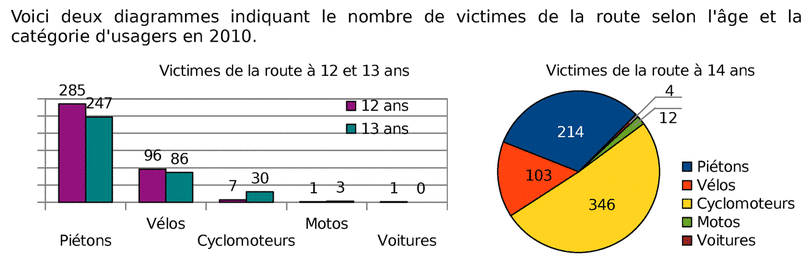
\includegraphics[scale=0.42]{img/IE-diagrammes.png} 
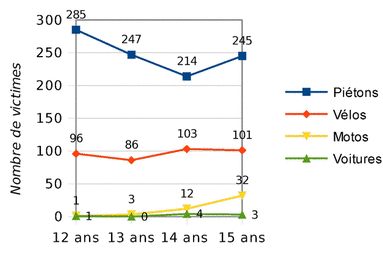
\includegraphics[scale=0.42]{img/IE-cart.png}
\end{center}
\begin{enumerate}
\item Quelle catégorie d'usagers de la route de 12 et 13 ans est le plus souvent victime d'accidents? \\ \gap*{Les usagers de 12 et 13 ans le plus souvent victime de la route sont \\ les piétons \hspace{11.7cm}}
\item Que permet de voir rapidement le diagramme circulaire?\\ \gap*{Le diagramme circulaire permet de voir que les cyclomoteurs sont les\\ plus victimes d'accident à 14 ans\hspace{7.5cm}}
\item Complète le tableau ci dessous
%\end{enumerate}
\begin{center}
\begin{tabular}{|c|c|c|c|c|c|}
\hline 
\thead{Nombre de \\ Victimes} & Piétons & Vélos & Cyclomoteurs & Motos & Voitures \\ 
\hline 
12 ans & \gap*[b]{285} & \gap*[b]{96} & \gap*[b]{7} & \gap*[b]{1} & \gap*[b]{1} \\ 
\hline 
13 ans & \gap*[b]{247} & \gap*[b]{86} & \gap*[b]{30} & \gap*[b]{3} & \gap*[b]{0} \\ 
\hline 
14 ans & \gap*[b]{214} & \gap*[b]{103} & \gap*[b]{346} & \gap*[b]{12} & \gap*[b]{4} \\ 
\hline 
15 ans & \gap*[b]{245} & \gap*[b]{101} & \gap*[b]{676} & \gap*[b]{32} & \gap*[b]{3} \\ 
\hline 
\end{tabular} 
\end{center}
%\begin{enumerate}
\item Quelle case ne peut pas être remplie? \gap*{Les cyclomoteurs de 15 ans victimes d'accidents}
\item Sachant que le nombre total de victimes de 15 ans est de 1057, calcule le nombre manquant et complète le tableau.
\end{enumerate}

\end{document}















